\documentclass[11pt,twoside,space]{ctexart}
\usepackage{CMC}
%%%%%%%%%%%%%%%%%%%%%%%%%%%%%%%%%%%%%%%%%%%%%%%%%%%%%%%%
\usepackage{float}
\usepackage[colorlinks=true,linkcolor=black]{hyperref}
\hypersetup{pdftitle={第九届中国大学生数学竞赛预赛试卷},
            pdfauthor={唐绍东},
            pdfsubject={2017年10月28日},
            pdfkeywords={大学生数学竞赛,白兔兔,预赛答案},}
%%%%%%%%%%%%%%%%%%%%%%%%%%%%%%%%%%%%%%%%%%%%%%%%%%%%%%%%
%\usepackage{blindtext}
\begin{document}\zihao{5}
\begin{center}\vspace{2mm}
	{\zihao{-2}\xingkai 第九届中国大学生数学竞赛预赛试卷}\\[2mm]
	{\zihao{4} $\left(\text{数学类, 2017年10月28日}\right)$}\\[0mm]
\end{center}
%输出"绝密"字样
{\heiti\zihao{-4} 绝密$\bigstar$启用前}\\[-17mm]%缩短"绝密"字样与总计分表之间的距离
\vspace*{2mm}
\begin{center}(14金融工程$-$白兔兔)\\[3mm] {\zihao{4}考试形式:\underline{~闭卷~}~\hspace{2mm}考试时间:\underline{~~150~~}分钟~\hspace{2mm}满分:~\underline{~~100~~}~分}\\
\vspace*{3.5mm}
{\zihao{-4}\begin{tabular}{|m{3em}<{\centering}|*{7}{m{3.5em}<{\centering}|}}\hline	
		题~号 & 一 & 二 & 三  & 四 & 五 & 六  &总~~分 \\\hline
		满~分 & 15 & 15 & 15  & 20 & 15 & 20  &\raisebox{0.4em}{100}\rule{0pt}{8mm}\\\hline
		得~分 &    &    &      &    &    &     &    \rule{0pt}{8mm} \\\hline
	\end{tabular}\\\vspace*{-1.5mm}
	\begin{equation*}\begin{aligned}
	\mbox{注意:}
	&1.\,\mbox{所有答题都须写在试卷密封线右边,写在其他纸上一律无效}.\hspace{12.0cm}\\
	&2.\,\mbox{密封线左边请勿答题,密封线外不得有姓名及相关标记}.\\
	&3.\,\mbox{如答题空白不够,可写在当页背面,并标明题号}.\\[-2mm]
	\end{aligned}\end{equation*}}	
\end{center}
\setlength{\marginparsep}{-0.8cm}
%%==================================================================
%%—————————————————————————————正文开始———————————————————————————————
%%==================================================================	

\vspace*{2.5em}
%\section{填空题\shusong{(本题满分20分, 共4小题, 每小题5分)}}
\dati{}{(本题15分)\;\;%\\[2mm]
在空间直角坐标系中,设单叶双曲面 $\Gamma$ 的方程为 $x^2+y^2-z^2=1$,设 $P$ 为空间的平面, 它交 $\Gamma$ 于一抛物线 $C$. 求该平面的法线与 $z$- 轴的夹角.\\} 


\newpage
%\section{\shusong{(本题满分15分)}}
\dati{}{(本题15分)\;\;
设 $\{a_n\}$ 是递增数列, $a_1>1$. 求证: 级数 $\textstyle\sum\limits_{n=1}^{\infty}\frac{a_{n+1}-a_n}{a_n\ln a_{n+1}}$ 收敛的充分必要条件是 $\{a_n\}$ 有界, 又问级数通项分母中的 $a_n$ 能否换成 $a_{n+1}$?}


\newpage
%\section{证明题\shusong{(本题满分15分)}}
\dati{}{(本题15分)\;\;
设 $\Gamma=\{W_1,W_2,\cdots,W_r\}$ 为 $r$ 个各不相同的可逆 $n$ 阶复方阵构成的集合. 若该集合关于矩阵乘法封闭(即, $\forall\,M,N\in\Gamma$, 有 $MN\in\Gamma$), 证明:  $\textstyle\sum\limits_{i=1}^{r}W_i=0$
当且仅当 $\textstyle\sum\limits_{i=1}^{r}\text{tr}(W_i)=0$, 其中 $\text{tr}(W_i)$ 表示 $W_i$ 的迹}


\newpage
%\section{\shusong{(本题满分20分)}}
\dati{}{(本题20分)\;\;
给定非零实数 $a$ 及实 $n$ 阶反对称矩阵 $A$ (即, $A$ 的转置 $A^T$ 等于 $-A$), 记矩阵有序对集合 $T$ 为\[T=\{(X,Y)|X\in\mathbb{R}^{n\times n},Y\in\mathbb{R}^{n\times n},XY=aI+A\},\]}\\[3ex]
其中 $I$ 为 $n$ 阶单位阵, $\mathbb{R}^{n\times n}$ 为所有实 $n$ 阶方阵构成的集合. 证明: 任取 $T$ 中两元: $(X,Y)$ 和 $(M,N)$ 必有 $XN+Y^TM^T\neq0$

\newpage
%\section{\shusong{(本题满分20分)}}
\dati{}{(本题15分)\;\;
设 $f(x)=\arctan x$, $A$ 为常数. 若
\[B=\lim_{n\to\infty}\bigg(\sum_{k=1}^{n}f\Big(\frac{k}{n}\Big)-An\bigg)\]}\\
存在, 求 $A,B$  



\newpage
%\section{\shusong{(本题满分15分)}}
\dati{}{(本题20分)\;\;
设 $f(x)=1-x^2+x^3\quad(x\in[0,1])$,\\
计算以下极限并说明理由\[\lim_{n\to\infty}\frac{\scaleobj{0.8}{\displaystyle\int_0^1}f^n(x)\ln(x+2)\dif x}{\scaleobj{0.8}{\displaystyle\int_0^1}f^n(x)\dif x}\]}











%%%%%%%%%%%%%%%%%%%%%%%%%%%%%%%%%%%%%%%%%%%%%%%%%%%%%%%%%%%%%%%%%%%%%
%------------------------------------结束--------------------------------------
%%%%%%%%%%%%%%%%%%%%%%%%%%%%%%%%%%%%%%%%%%%%%%%%%%%%%%%%%%%%%%%%%%%%%
\clearpage

\end{document}




%  合并为一面双页
%  先保存再编译
\documentclass{article}
\usepackage{pdfpages}
\usepackage[paperwidth=40cm,paperheight=27.5cm]{geometry}
\begin{document}
	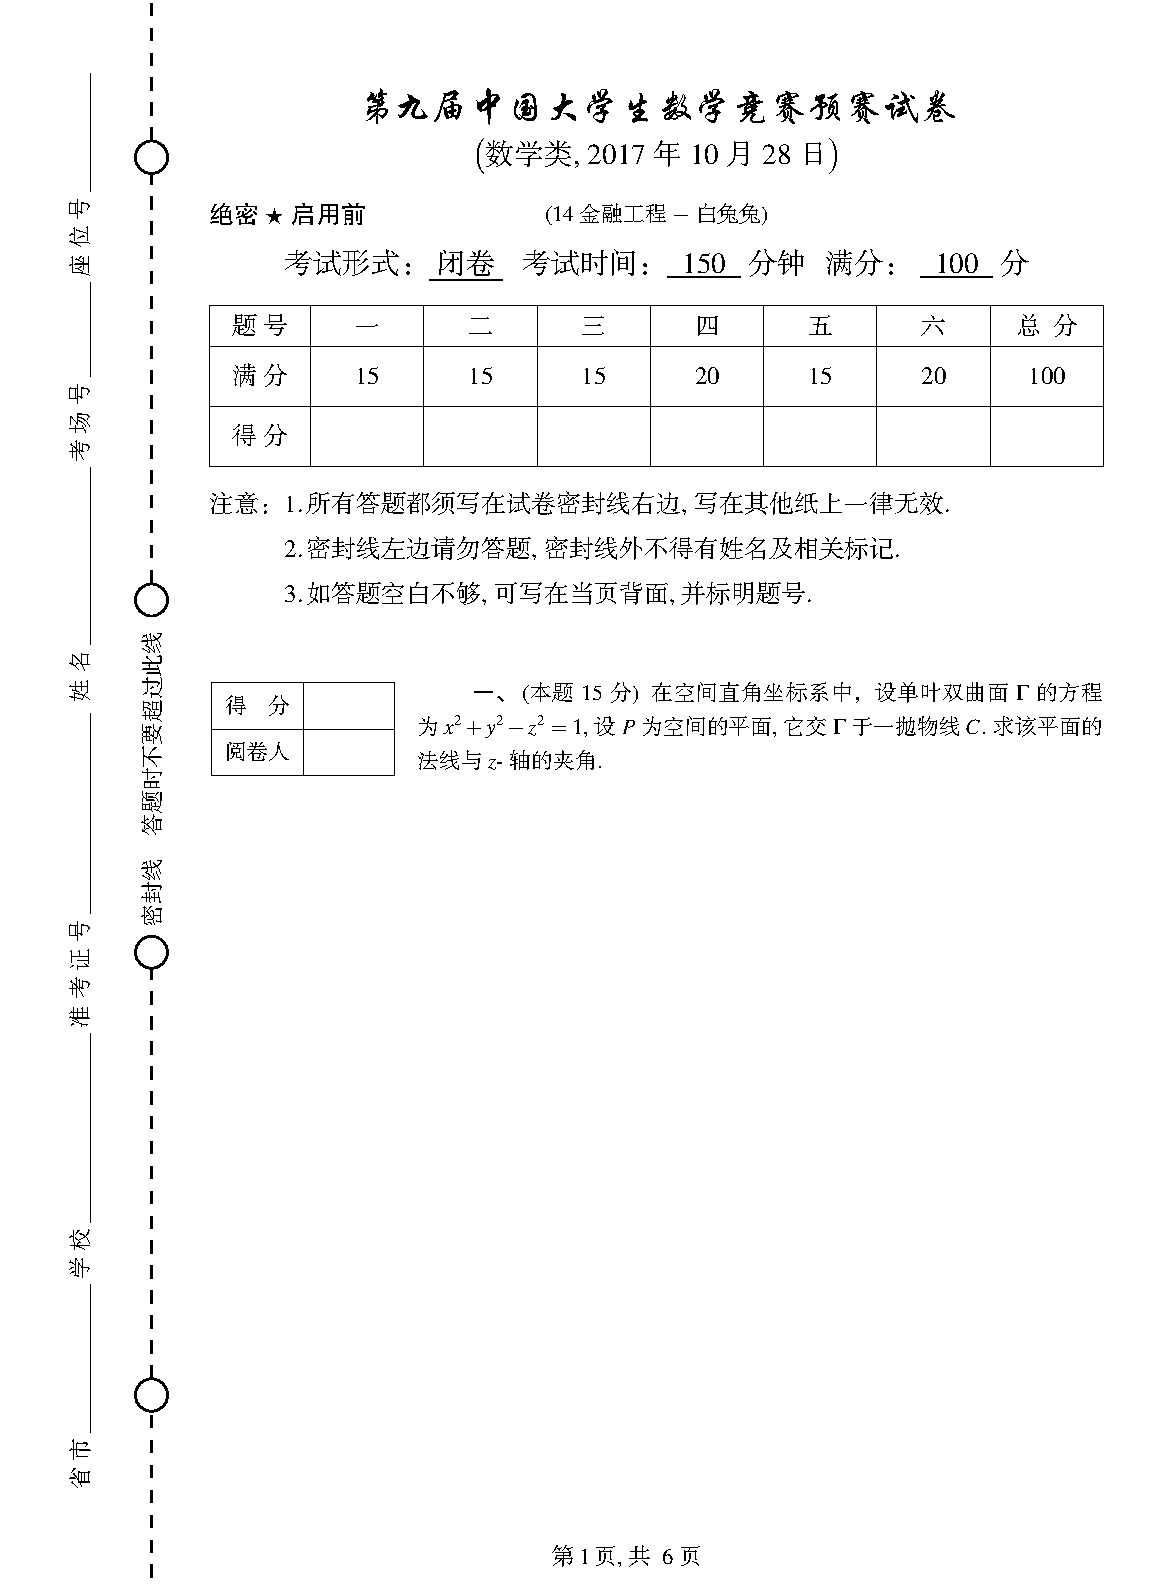
\includepdf[pages=1-6,nup=2x1,scale=1,offset=3mm 0mm,column,delta=-10 -0mm]{17mathshijuan.pdf}	
\end{document}

